% TeXplates/Mathematics.tex
% v0.2.2
% https://github.com/HoyanMok/TeXplates
\documentclass[openany]{book} 
% \documentclass{ctexbook} 如果用中文
% \documentclass[10pt,a4paper]{ctexart}  字体大小和纸张大小,默认分别为10pt和letterpaper
% 五号 = 10.5pt,小四=12pt,四号=14pt
% 其他可选参量如twocolumn, 两行排版
\usepackage{../TeXplatesMathematics}
\usepackage{xeCJK}

\addbibresource{PointSetTopology.bib} % 把这里改成实际的文件名

\title{Point Set Topology}
\author{Hoyan Mok}
\begin{document}
\pagenumbering{Alph}
\maketitle
\frontmatter

\tableofcontents
\mainmatter
\chapter{Topological Spaces and Continuous Mappings}
\section{Metric Space}
\begin{definition}\label{metric_def}
function
\begin{align}\label{metric}
	\indexmath[d]{d}\colon X^2\to\mathbb{R}
\end{align}
$\forall x_1,x_2,x_2\in X$ satisfied: 
\begin{conditionlist}[label=\alph*)]
	\item	$d(x_1,x_2)=0\Leftrightarrow x_1=x_2$;
	\item	$d(x_1,x_2)=d(x_2,x_1)$ (symmetry);
	\item	$d(x_1,x_3)\leqslant d(x_1,x_2)+d(x_2,x_3)$ (Triangle inequality),
\end{conditionlist}
is called a \indexbf{metric} or \indexbf{distance} in $X$. Such $X$ is said to be equiped with metric $d$, $(X,d)$ is called a \indexbf{metric space}.
\end{definition}

Some examples:
\begin{itemize}
\item $(\mathbb{R}^n;d_p)$, where $d_p(x_1,x_2)=\left(\sum^n_{i=1}\left|x^i_1-x^i_2\right|^p\right)^{1/p}$, while $d_\infty(x_1,x_2)=
\max\limits_{1\leqslant i\leqslant n}
\left|x^i_1-x^i_2\right|$.
\item Similarly we can define metric spaces as $(C[a,b];d_p)$ or $C_p[a,b]$. $d_p(f,g)=\left(
	\int^b_a\left|f-g\right|^p\,\mathrm{d}x
\right)^{\frac{1}{p}}$. $C_\infty$ is called a \textbf{Chebyshev metric}\index{Chebyshev metric}.
\item On class $\mathfrak{\tilde{R}}[a,b]$ over $\mathfrak{R}[a,b]$ similar metric can be defined. Functions are considered of one same class if they are equivalent expect on a set not larger than null set. 
\end{itemize}

\indexbf{Hilbert space} denoted by $(\indexmath[H]{\mathbb{H}}; d)$ is defined as:

\begin{align}
	\mathbb{H}=\left\{ 
		x=(x_1,x_2,\cdots) \mid \forall i\in \mathbb{Z}_+\left( 
			\forall x_i\in \mathbb{R}\wedge \sum^\infty_{i=1} x_1^2 < \infty\right)\right\}
\end{align}
equiped with a metirc $d$:

\begin{align}
	d\colon \mathbb{H}^2\to \mathbb{R}; \,x,y\mapsto \sqrt {\sum^\infty_{i=1} (x_i-y_i)^2 }.
\end{align}

To justify this definition, we need to introduce a lemma:
\begin{lemma}\label{Schwarz_inequality}
\begin{align}\label{Schwarz}
	\forall n\in\mathbb{Z}\forall \bv u\in\mathbb{R}^n\forall \bv v\in\mathbb{R}^n\left(
		\sum^n_{i=1} u_iv_i \leq \sqrt{ \sum^n_{i=1} u_i^2}\sqrt{ \sum^n_{i=1} v_i^2}\right)
\end{align}
This is called \indexbf{Schwarz inequality}.
\end{lemma}
\begin{proof}
If $\forall i=1,\cdots,n ( v_i=0)$ the equivalence has already been satisfied, therefore the following considers the situation that $\exists i\in \{1,\cdots n\}( v_i\neq 0)$. $\forall \lambda \in\mathbb R$, the quadratic polynomial of $\lambda$
\begin{align*}
	\sum ^n_{i=1} (u_i+\lambda v_i)^2 = 
		\sum ^n_{i=1} u_i^2 +2\lambda \sum ^n_{i=1} u_iv_i + \lambda^2 \sum ^n_{i=1} v_i^2 \geq 0
\end{align*}
has at most one root. Hence $\Delta \leq 0$ will lead to the inequality \ref{Schwarz}.
\end{proof}

Apply this inequality to $\sum ^n_{i=1} ( u_i+v_i)^2 = 
	\sum ^n_{i=1} u_i^2 +\sum ^n_{i=1}  v_i^2 +2\sum ^n_{i=1}  v_i\sum ^n_{i=1} u_i$ we can get
\begin{align*}
	\sum ^n_{i=1} ( u_i+v_i)^2 \leq 
		\sum ^n_{i=1} u_i^2 +\sum ^n_{i=1}  v_i^2 +
			2\sqrt{ \sum^n_{i=1} u_i^2}\sqrt{ \sum^n_{i=1} v_i^2} = \left(
				\sqrt{ \sum^n_{i=1} u_i^2}+\sqrt{ \sum^n_{i=1} v_i^2} \right)^2 ,
\end{align*}
in which substitude $u_i,v_i$ by $x_i-y_i, x_i+y_i$ will result in triangle inequality. The inequality holds as the $n$ limits to $+\infty$.

\begin{definition}
Let $(X,d)$ be a metric space, the \indexbf{distant} between a non-empty set $\varnothing\neq A\in \mathscr P(X)$ and a point $x$ is defined as:
\begin{align*}
	d(A,x) = \inf \{d(x,y)\mid y\in A\},
\end{align*}
and we let $d(x,A) = d(A,x)$. 
Also, the \indexbf{distant} between two non-empty sets $A,B$ is defined as:
\begin{align*}
	d(A,B) = \inf \{d(x,y)\mid x\in A\wedge y\in B\}.
\end{align*}
\end{definition}

A metric space $(X,d)$ is called \indexbf{discrete} if 
\begin{align*}
	\forall x\in X\left(
		\exists \delta_x\in \mathbb{R}_+ \big(
			\forall y \in X(
				y\neq x\to d(x,y)>\delta_x)\big)\right) .
\end{align*}

\begin{lemma}\label{quadruple_inequality}
If $(X,d)$ is a metric space, then $\forall a,b,u,v $, $\left| d(a,b) - d(u,v) \right| \leq d(a,u)+d(b,v) $.
\end{lemma}
\begin{proof}
	Without loss of generality, we assume that $d(a,b) > d(u,v)$. According to the triangle inequality (see def. \ref{metric_def}), $d(a,b) \leq d(a,u)+d(u,v)+d(v,b)$, which is to prove.  
\end{proof}

\begin{definition}\label{delta_ball}
$\delta\in\mathbb{R}_+$, $a\in X$. Set
\[
	B(a;\delta)=\{x\in X \mid d(a,x)<\delta\}
\]
is then called a \indexbf{ball} with centre $a\in X$, and a radius of $\delta$, or a \indexbf{$\delta$-ball} of point $a$.
\end{definition}

\begin{definition}\label{open_set_metric}
An \indexbf{open set} $G\subset X$ in metric space $(X,d)$ satisfies: $\forall x\in G$, $\exists B(x;\delta)$, s.t. $B(x;\delta)\subset G$.
\end{definition}

\begin{definition}\label{closed_set_metric}
A set $F\subset X$ in metric space $(X,d)$ is said to be a \indexbf{closed set} if its complement $\complement_X(F)$ is open.
\end{definition}

It can be proved that $\varnothing$ and $X$ itself is both open and closed.

\begin{proposition}\label{open_set_pro}
\begin{enumerate}[label=\alph*)]
\item An infinite union of open sets is an open set.
\item A finite intersection of open sets is an open set.
\item A finite union of closed sets is a closed set.
\item An infinite intersection of closed sets is a closed set.
\end{enumerate}
\end{proposition}
\begin{proof}
\begin{enumerate}[label=\alph*)]
	\item If open sets $G_\alpha\subset X,\forall\alpha\in A$, $\forall a\in\bigcap\limits_{\alpha\in A}G_\alpha$, $\exists\alpha_0\in A$, $a\in G_{\alpha_0}$, $\exists B(a;\delta)\subset G_{\alpha_0}\subset \bigcap\limits_{\alpha\in A}G_\alpha$.
	\item Open sets $G_1\cup G_2\subset X$, $a\in G_1\cap G_2$, therefore $\exists\delta_1,\delta_2\in\mathbb{R}_+$, $B(a;\delta_1)\subset G_1,B(a;\delta_2)\subset G_2$, without loss of generality, let $\delta_1\geq\delta_2$, 那么$a\in B(a;\delta_1)\cap B(a;\delta_2)=B(a;\delta_2)\subset G_1\cap G_2$.
	\item Just consider $\complement_X
		\left(\bigcap_{\alpha\in A}F_\alpha\right)
		=\bigcup_{\alpha\in A}\complement_X(F_\alpha)$ and a).
	\item Similarly, $\complement_X\left(F_1\cup F_2\right)=\complement_X(F_1)\cap\complement_X(F_2)$.
	
\end{enumerate}
\end{proof}

\section{Topological Space}
\begin{definition}\label{topological_space}
We say $X$ is equiped with a \indexbf{topological space} or equiped with \indexbf{topology} if we assigned a $\indexmath[T]{\mathscr{T}}\subset 2^X$, which has got the following propoties:
\begin{conditionlist}[label=\alph*)]
	\item $\varnothing\in\mathscr{T}; X\in\mathscr{T}$.
	\item $\forall\alpha\in A(
		G_\alpha\in\mathscr{T})\to 
			\bigcup\limits_{\alpha\in A}G_\alpha\in\mathscr{T}$.
	\item $G_1\in\mathscr{T}\wedge G_2\in\mathscr{T}\to G_1\cap G_2\in \mathscr{T}$.
\end{conditionlist}

Then we call $(X,\mathscr{T})$ a \indexbf{topological space}. Every $G\in \mathscr{T}$ is called an \indexbf{open set}. 
\end{definition}

\begin{definition}\label{induced_topology}
A topology $\mathscr{T}_d$ insisting of the open sets in a metric space $( X, d)$ is called a \indexbf{topology induced by metric} $d$.
\end{definition}

A trivial example of topological space is \indexbf{trivial topology}, which consists only of empty set and the space itself, i.e.\ $\mathscr{T}=\{\varnothing, X\}$. Another trivial example of topological space is \indexbf{discrete topology}, which consists of all the subsets of the space i.e.\ $\mathscr{T} = 2^X$.

A \indexbf{cofinite space} is a base set $X$ equiped with a topology $\mathscr{T}$ defined as follows:
\begin{align}\label{cofinite_space}
	\mathscr{T} = \{ U\in 2^X\mid U=\varnothing \vee \complement_X U \text{ is finite} \}
\end{align}
\begin{proposition}
The set $\mathscr{T}$ under definition \ref{cofinite_space} is a topology.
\end{proposition}
\begin{proof}
\begin{enumerate}[label=\alph*)]
\item $\varnothing \in \mathscr{T}$, $X\in\mathscr T$.
\item $\forall i \in I \left(
	\left|\complement_X  A_i\right| \in \mathbb N\right) \to
		\forall i_0\in I\left(
			\left| \bigcap_{i\in I} \complement_X A_i\right| \leq 
				\left|\complement_X A_{i_0}\right|\right)$, therefore $\bigcup_{i\in I}  A_i \in \mathscr T$.
\item $\forall A\in \mathscr T \forall B \in \mathscr T(
	A\cap B=\varnothing\in \mathscr{T} \vee
		\complement_X (A\cap B) = \complement_X A\cup \complement_X B \text{ is finite} )$, 
	therefore $\forall A\in \mathscr T \forall B \in \mathscr T(
		A\cap B \in \mathscr T)$.
\end{enumerate}
\end{proof}

Similarly, \indexbf{countable complement space} can be defined.

Let $X$ be equiped with two topology $\mathscr T_1, \mathscr T_2$. $\mathscr T_1\cup \mathscr T_2$ is possibly not a topology of $X$. For example, $\mathscr T _1 = \{ (x,+\infty) \mid x\in\mathbb R\}\cup\{ \varnothing,\mathbb R\}$ and $\mathscr T_2 = \{ (-\infty, y) \mid y\in\mathbb R\}\cup\{ \varnothing,\mathbb R\}$ are both topologies of $\mathbb R$, but there union $T_1\cup T_2$ is not. 

\begin{theorem}
Let $X$ be equiped with two topology $\mathscr T_1, \mathscr T_2$. Their intersection $\mathscr T_1\cap \mathscr T_2$ is also a topology on $X$.
\end{theorem}
\begin{proof}
\begin{enumerate}[label=\alph*)]
\item $\{\varnothing, X\} \subseteq \mathscr T_1\wedge 
	\{\varnothing, X\} \subseteq  \mathscr T_2 \to 
		\{\varnothing, X\}\subseteq \mathscr T_1\cap \mathscr T_2$.
\item $\forall\alpha\in A(
		G_\alpha\in\mathscr T_1\cap \mathscr T_2)\to 
			\bigcup\limits_{\alpha\in A}G_\alpha\in\mathscr{T}_1 \wedge \bigcup\limits_{\alpha\in A}G_\alpha\in\mathscr{T}_2$. 
\item $\forall G_1\in \mathscr T_1\cap \mathscr T_2 \forall G_2 \in \mathscr T_1\cap \mathscr T_2 \big(
		G_1\cap G_2 \in \mathscr T_1 \wedge G_1\cap G_2\in\mathscr T_2\big)$			
\end{enumerate}
\end{proof}

\begin{definition}\label{matrization}
Let $(X, \mathscr T)$ be a topological space. If there exists a metric $d\colon X^2\to \mathbb R$ s.t.\ $(X, \mathscr T)$ is induced by $d$ then call $(X, \mathscr T)$ a \indexbf{metrizable space}, $(X, d)$ is its \indexbf{metrization}.
\end{definition}

\section{Neighbourhood}
\begin{definition}\label{neighbourhood}
Let $(X,\mathscr T)$ be a topological space. A set $U(x)$ is said to be a \indexbf{neighbourhood} of a point $x\in X$ if $\exists G\in \mathscr T(G\subseteq U(x)\wedge x\in G)$. 
If $U(x)\in \mathscr T$, it is called an \indexbf{open neighbourhood}.
Subset class $\{U(x)\subseteq X\mid U(x) \text{ is a neighbourhood of } x\}$ is called the \indexbf{neighbourhood system} of point $x$, denoted by $\mathscr U_x$
\end{definition}

\begin{theorem}\label{open_iff_neighbourhood}
Let $(X,\mathscr T)$ be a topological space, $U$ is a subset of $X$. 
$U$ is an open set \emph{iff} $\forall x\in U$, $U$ is a neighbourhood of $x$.
\end{theorem}
\begin{proof}
The necessity is trivial. 
$\forall x\in U\exists V(x)$ s.t.\ $V(x)$, being a subset of $U$, is an open neighbourhood of $x$. 
By definition of topology, $\bigcup\limits_{ x\in U}V(x) \in \mathscr T$. 
$\forall x\in U( x\in \bigcup\limits_{ x\in U}V(x) ) \to U\subseteq V$, 
while $\forall x\in U (V( x)\subseteq U)\to \bigcup\limits_{ x\in U}V(x) \subseteq U$, 
therefore $U=\bigcup\limits_{ x\in U}V(x) \in \mathscr T$.
\end{proof}

\begin{theorem}
Let $(X,\mathscr T)$ be a topological space, $\mathscr U_x$ is a neighbourhood system of point $x\in X$.
\begin{align*}
	\forall U\in \mathscr U_x\forall V\in \mathscr U_x( U\cap V\in \mathscr U_x)
\end{align*}
\end{theorem}
\begin{proof}
$\forall U\in \mathscr U_x\forall V\in \mathscr U_x\exists U_0\in \mathscr T\exists V_0\in \mathscr T(U_0\subseteq U\wedge V_0\subseteq V\wedge x\in U_0\cap V_0 )$, By definition of topology, $\mathscr T\ni U_0\cap V_0\subseteq U\cap V$. 
\end{proof}

In history topologies were once built on neighbourhood systems. The following theorem shows the way.
 
\begin{theorem}\label{topology_built_on_neighbourhood}
Let $X$ be a set and $\forall x \in X$ a collection of subsets $\mathscr U_x \in \mathscr P(X)$ is appointed, satisfying:
\begin{conditionlist}[label=(\arabic*)]
\item $\forall x\in X\big(
	\mathscr U_x \neq \varnothing \wedge
		\forall U\in \mathscr U_x (x\in U)\big)$; 
\item $\forall x\in X\forall U\in\mathscr U_x\forall V\in\mathscr U_x (
	U\cap V\in \mathscr U_x)$;
\item $\forall x\in X\forall U\in\mathscr U_x\forall V\in \mathscr P(X)( 
	U\subseteq V \to V\in \mathscr U_x)$;
\item $\forall x\in X\forall U\in\mathscr U_x\exists V\in\mathscr U_x \big(
	V\subseteq U \wedge \forall y\in V(V\in \mathscr U_y)\big)$,
\end{conditionlist}
then there exists only one topology $\mathscr T$ on $X$ s.t.\ $\forall x\in X$, $\mathscr U_x$ is the neighbourhood system of $x$ in $(X,\mathscr T)$.
\end{theorem}
\begin{proof}
Let $\mathscr T = \{G\in \mathscr P(X) \mid \forall x\in G( G\in \mathscr U_x)\}$.
\begin{enumerate}[label=\alph*)]
\item Obviously $\varnothing \in \mathscr T$. 
	Since the condition (1) and the condition (3) in theorem \ref{topology_built_on_neighbourhood}, $X\in \mathscr T$.
\item Let $A, B\in \mathscr T$. Consider the condition (2) in theorem \ref{topology_built_on_neighbourhood} applied to $x\in A\cap B$.
\item Let $\forall i\in I( G_i \in \mathscr T)$. 
$\forall x\in \bigcup_{i\in I} G_i$, there must exists a $i\in I$ s.t.\ $x\in G_i$ and $G_i \in \mathscr U_x$. 
Since the condition (3) in theorem \ref{topology_built_on_neighbourhood}, $G_i \subseteq \bigcup_{i\in I} G_i$ has implied $\bigcup_{i\in I} G_i \in \mathscr U_x$.
\end{enumerate}
These tells that $\mathscr T$ is a topology on $X$.

The condition (4) in theorem \ref{topology_built_on_neighbourhood} tells that there always exists a $G\subset U$ for all $x\in X$ and $U\in \mathscr U_x$ s.t.\ $G\in \mathscr T$. Therefore $\mathscr U_x$ must be a subset of the neighbourhood system of $x$. 

For all neighbourhood $U$ of $x\in X$, there must be a open neighbourhood subset $G\subseteq U$, which is also a member of $\mathscr U_x$. Since the condition (3) in theorem \ref{topology_built_on_neighbourhood}, $U\in \mathscr U_x$. Therefore the neighbourhood system of $x$ must be a subset of $\mathscr U_x$. 

Therefore, $\mathscr U_x$ is the neighbourhood system of $x$.

Now prove the uniqueness. Let there be another topology $\mathscr T '$.
Since theorem \ref{open_iff_neighbourhood}, 
$\forall U\big(
	G\in \mathscr T' \leftrightarrow 
		\forall x\in G(
			G\in \mathscr U_x)\big)$. 
Therefore $\mathscr T' = \mathscr T$.
\end{proof}

\section{Continuous Mappings}
\begin{definition}\label{continuousness}
A mapping $f\colon X\to Y$, where $X$,$Y$ is respectively equiped with topology $\mathscr{T}_X$,$\mathscr{T}_Y$, is said to be \indexbf{continuous} at $x_0\in X$ (let $y_0 = f( x_0 ) \in Y$), if $\forall U( y_0 )$, $\exists U( x_0 )$ s.t. $f( U(x_0) )\subset U( y_0 )$. It is \indexbf{continuous} in $X$ if it is continuous at each point $x\in X$. 
\end{definition}

The set of continuous mappings from $X$ into $Y$ can be denoted by $C(X,Y)$ or $C(X)$ when $Y$ is clear. 

It can be easily proved that an identify function $e_X\colon X\to X$ where $X$ is equiped with a topology $\mathscr T$ is a continuous function.

\begin{theorem}\label{criterion_continuity} (\indexbf{criterion of continuity})

Let $(X, \mathscr T)$, $(Y; \mathscr S)$ be two topological space. A mapping $f \colon X \to Y$ is continuous \emph{iff}
\begin{align*}
	\forall V\in \mathscr S\big(
		\exists U \in \mathscr T(
			U=f^{-1}(V) ) \big).
\end{align*}
\end{theorem}
\begin{proof}
$\rightarrow$: It is obvious if $f  ^{-1}(G_Y) = \varnothing$. 
If $f  ^{-1}(G_Y) \neq \varnothing$ and $\forall x_0 \in f  ^{-1}(G_Y)$, 
since $f \in C(X,Y)$, for $G_Y \in \mathscr S$, $\exists U( x_0) $ s.t $f ( U( x_0)) \subset G_Y$. 
Also notice that $f ( U( x_0)) \subset G_Y \Rightarrow U( x_0) \subset f  ^{-1}(G_Y)$, therefore $f  ^{-1}(G_Y) $ is open (Theorem \ref{open_iff_neighbourhood}).

$\leftarrow$: $\forall x_0 \in X$, let $y_0 = f ( x_0)$, $f ^{-1} ( U( y_0)) \in \mathscr{T}$ if $U(y_0) \in \mathscr S\cap \mathscr U_{y_0}$.
Notice that $x_0 \in f ^{-1} ( U( y_0))$, $ f ^{-1} ( U( y_0))$ is a neighbourhood of $x_0$, therefore $f \in C( X, Y) $.
\end{proof}

\begin{theorem}
	Let $(X, \mathscr T_X)$, $(Y, \mathscr T_Y)$, $(Z, \mathscr T_Z)$ be topological spaces.
	If $f\colon X\to Y$ and $g\colon Y\to Z$ are both continuous, $g\circ f\colon X\to Z$ is also continuous. 
\end{theorem}
\begin{proof}
\begin{align*}
	\forall W\in \mathscr T_Z\left(
		g^{-1} (W)\in \mathscr T_Y\right) \rightarrow 
			\forall W\in \mathscr T_Z\left(
				f^{-1}\big( 
					g^{-1} (W)\big)\right)
\end{align*}
Since $f^{-1}\big(  g^{-1} (W)\big) = ( g\circ f)^{-1} (W)$, the theorem has been proved.
\end{proof}

\begin{definition}\label{homeomorphism}
$(X,\mathscr{T}_X)$ and $(Y,\mathscr{T}_Y)$ are both topological spaces. A bijective mapping $f \colon X\to Y$ is a \indexbf{homeomorphism} if $f \in C( X, Y) \wedge f ^{ -1} \in C( Y, X)$. 
\end{definition}
\begin{definition}\label{homeomorphic}
Two topological spaces $(X,\mathscr{T}_X)$ and $(Y, \mathscr{T}_Y)$ are said to be \indexbf{homeomorphic} if there exists a homeomorphism $f \colon X\to Y$.
\end{definition}

Homeomorphic topological spaces are identical with respect to their topological propoties since the Theorem~\ref{criterion_continuity} has shown that their open sets correspond to each other. In fact homeomorphic relations are equivalent relations.

\begin{lemma}[Gluing lemma]%
	\label{lemma: gluing}
	$\mathscr F = \{F_i \mid \complement_X F_i \in \mathscr T, i \in n\}$, $X \subseteq {\cup \mathscr F}$, $f \colon X \to Y$. 
	If $\forall F \in \mathscr F$, $f \vert_F \in C(F, Y)$, then $f \in C(X, Y)$.
\end{lemma}
\begin{proof}
	$\forall F_Y ( \complement_Y F_Y \in \mathscr T)$, 
	\begin{equation*}
		f^{-1}(F_Y) = \bigcup_{i \in n} F_i \cap f^{-1}(F_Y) = \bigcup_{i \in n} f^{-1} \vert_{F_i} (F_Y).
	\end{equation*}

	The finite intersection of closed sets are also closed, while the pre-image of a closed set is also closed (when mapping is continuous). 
\end{proof}

\section{Closure}
\begin{definition}\label{accumulation_point}
Let $X$ be a topological space and $A$ be a subset of $X$. Let $x\in X$.
If $\forall U\in \mathscr U_x \big(
	U\cap (A-\{x\}) \neq \varnothing\big)$, 
then $x$ is called a \indexbf{accumulation point}, \indexbf{cluster point} or \indexbf{limit point} of $A$. 
The set $A' := \{x\in X\mid x\text{ is a accumulation point of } A\}$ is called the \indexbf{derived set} of $A$.
A point $a\in A$ is called a \indexbf{isolated point} of $A$ if $a\notin A'$.
\end{definition}

\begin{theorem}\label{propoties_derived}
Let $X$ be a topological space and $A$, $B$ be subsets of $X$. 
1) $A\subseteq B \to A'\subseteq B'$; 
2) $(A\cup B)' = A'\cup B'$;
3) $(A')' \subseteq A\cup A'$.
\end{theorem}
\begin{proof}
\begin{enumerate}[label=\arabic*)]
\item When $A\subseteq B$, $U\cap (A-\{x\}) \subseteq U\cap (B-\{x\})$.
\item $(A\cup B)' = \{x\in X\mid \forall U\in \mathscr U_x \big(
	U\cap (A\cup B-\{x\}) \neq \varnothing\big)\}$. 
Also $U\cap (A\cup B - \{x\}) = U\cap (X-\{x\})\cap (A\cup B) = (U\cap A-\{x\})\cup (U\cap B-\{x\})$.
\item If $x\notin A\cup A'$, then $\exists G\in \mathscr U_x\cap \mathscr T \big(
	G\cap (A-\{x\}) = G\cap A = \varnothing\big)$. 
$\forall y \in G$, $G$ itself is a neighbourhood of $y$ that $G\cap (A-\{y\}) = G\cap A =\varnothing$, therefore $y\notin A'$. 
This means that $G$ is a neighbourhood of $x$ that $G\cap (A'-\{x\}) = G\cap A' =\varnothing$, i.e.\ $x\notin (A')'$.
\end{enumerate}
\end{proof}

\begin{definition}\label{closed_set}
Let $(X,\mathscr T)$ be a topological space and $F$ be a subset of $X$. $F$ is said to be \indexbf{closed} \emph{iff} $\complement_X (F) \in \mathscr T$. The collection all closed sets is denoted by $\mathscr F$.
\end{definition}

\begin{theorem}\label{closed_iff_accumulation}
Let $(X,\mathscr T)$ be a topological space and $F$ be a subset of $X$. $F$ is closed \emph{iff} $ F'  \subseteq F$.
\end{theorem}
\begin{proof}
$\to$: 
If $x\notin F$ then $x\in \complement_X (F)$, which is open in $(X,\mathscr T)$. 
Then $\complement_X (F)$ is a neighbourhood that $\complement_X (F) \cap (F-\{x\}) = \complement_X (F) \cap F =\varnothing$, i.e.\ $x\notin F'$.

$\leftarrow$:
$\forall x\notin F(x\notin F')$, then there exists an open neighbourhood $U$ of $x$ that $U\cap F = \varnothing$, then $\complement_X (F)$ is always a neighbourhood of its elements, since theorem \ref{open_iff_neighbourhood}, $\complement_X (F) \in \mathscr T$.
\end{proof}

\begin{definition}\label{closure}
Let $(X,\mathscr T)$ be a topological space and $A$ be a subset of $X$. Set $\overline A := A\cup A'$ is called a \indexbf{closure} of $A$.
\end{definition}

\begin{theorem}\label{closure_neighbourhood}
Let $(X,\mathscr T)$ be a topological space and $A$ be a subset of $X$. Let $x\in X$.
\[
	x\in \overline A \leftrightarrow
		\forall U\in\mathscr U(x)(
			U\cap A\neq \varnothing).
\]
\end{theorem}
\begin{proof}
$\to$: If $x\in A$ then $\{x\}\subseteq U\cap A$, 
else if $x\in A'$ then $U\cap A \supset (U-\{x\})\cap A \neq \varnothing$.

$\leftarrow$: 
If $\exists U\in\mathscr U(x)\big(
	(U-\{x\})\cap A= \varnothing\big)\wedge x\notin A$, 
then there exists a $U\in \mathscr U(x)$ s.t.\ $U\cap A=\varnothing$. 
\end{proof}


\begin{theorem}\label{closed_iff_closure}
Let $(X,\mathscr T)$ be a topological space and $A$ be a subset of $X$. 
$A$ is closed in $(X,\mathscr T)$ \emph{iff} $A=\overline A$.
\end{theorem}
\begin{proof}
Since theorem \ref{closed_iff_accumulation}, $A$ is closed iff $A'\subseteq A$, which iff $A = A\cup A' = \overline A$.
\end{proof}

\begin{corollary}\label{closure_closed}
Let $(X,\mathscr T)$ be a topological space and $A$ be a subset of $X$. 
$\overline A$ is always closed.
\end{corollary}
\begin{proof}
Since (3) of theorem \ref{propoties_derived}, $\overline{\overline A} = \overline A$.
\end{proof}

\begin{lemma}\label{subset_closure}
Let $(X,\mathscr T)$ be a topological space and $A$, $B$ be subsets of $X$.
$A\subseteq B \to \overline A\subseteq \overline B$.
\end{lemma}
\begin{proof}
$A\subseteq B \to A'\subseteq B'$ ((1) of theorem \ref{propoties_derived}), so $A\cup A'\subseteq B\cup B'$, i.e.\ $\overline A\subseteq \overline B$.
\end{proof}

We can say that the closure of a set is the smallest closed set containing it, as long as we prove the following theorem:

\begin{theorem}
Let $(X,\mathscr T)$ be a topological space and $A$ be a subset of $X$.
\begin{align*}
	\overline A = \bigcap_{F\in \mathscr F \wedge A\subseteq F} F.
\end{align*}
\end{theorem}
\begin{proof}
Since $\overline A$ itself is closed (corollary \ref{closure_closed}), $\bigcap_{F\in \mathscr F \wedge A\subseteq F} F \subseteq \overline A$. 
On the other hand, $\bigcap_{F\in \mathscr F \wedge A\subseteq F} F$ is closed, so $\overline{\bigcap_{F\in \mathscr F \wedge A\subseteq F} F} = \bigcap_{F\in \mathscr F \wedge A\subseteq F} F$.
Therefore, $A\subseteq \bigcap_{F\in \mathscr F \wedge A\subseteq F} F \to \overline A \subseteq \bigcap_{F\in \mathscr F \wedge A\subseteq F} F$ (Lemma \ref{subset_closure}). 
\end{proof}

\begin{theorem}
Let $(X,d)$ be a metric space and $A$ be a non-empty subset of $X$.
\begin{enumerate}[label=\arabic*)]
\item $\forall x\in X$, $x\in A' \leftrightarrow d(x,A-\{x\}) = 0$.
\item $\forall x\in X$, $x\in \overline A \leftrightarrow d(x,A)=0$.
\end{enumerate}
\end{theorem}
\begin{proof}
\begin{enumerate}[label=\arabic*)]
\item We have $x\in A' $ \emph{iff} $\forall \varepsilon\in \mathbb R_+\big(
	B (x,\varepsilon) \cap (A-\{x\}) \neq \varnothing\big)$, 
which is established \emph{iff} $\forall \varepsilon \in \mathbb R_+\exists y\in A-\{x\}\big(
	d(x,y) <\varepsilon\big)$.
\item We only need to substitude $A-\{x\}$ with $A$ in 1).
\end{enumerate}
\end{proof}

\begin{theorem}
Let $(X, \mathscr T)$ and $(Y,\mathscr S)$ be two topological spaces, and $f\colon X\to Y$. Note the collections of closed sets in $X$ and $Y$ by $\mathscr F_X$, $\mathscr F_Y$.
The statements below are equivalent:
\begin{conditionlist}[label=(\arabic*)]
\item $f\in C(X,Y)$.
\item $\forall F\in\mathscr F_Y \big(
	f^{-1} (F) \in \mathscr F_X\big)$.
\item $\forall A\in \mathscr P(X) \big(
	f(\overline A) \subseteq \overline{ f(A)}\big)$.
\item $\forall B\in \mathscr P(Y) \big(
	\overline{f^{-1} (B)}\subseteq f^{-1} (\overline B) \big)$.
\end{conditionlist} 
\end{theorem}
\begin{proof}
(1) $\to$ (2): Only to notice that $f^{-1} (\complement_Y F ) =\complement_X f^{-1} (F)$. 

(2) $\to$ (3): $\forall A \in \mathscr P(X)$ we have $f(A) \subseteq \overline{f(A)}$, so $A \subseteq f^{-1} \big(
	\overline{f(A)}\big)$. 
By (2) we know that $f^{-1} \big(\overline{f(A)}\big)$ is closed, therefore 
$\overline A \subseteq \overline{f^{-1} \big(\overline{f(A)}\big)} 
	= f^{-1} \big(\overline{f(A)}\big)$, so $f(\overline A) \subseteq \overline {f(A)}$.
	
(3) $\to$ (4): By (3) we know that $\forall B\in \mathscr P(Y)$, 
$f\big(\overline{f^{-1}(B)}\big) \subseteq \overline{f(f^{-1}(B))}$. 
Also $f(f^{-1}(B)) \subseteq B$ (equality satisfied when $f$ is surjective), 
then $f\big(\overline{f^{-1}(B)}\big) \subseteq \overline B$, 
so $\overline{f^{-1}(B)} \subseteq f^{-1} (\overline B)$.

(4) $\to$ (1): $\forall G\in \mathscr S$, $\complement_Y G \in \mathscr F_Y$, so by (3), we have
\begin{align*}
	\overline {\complement_X f^{-1}(G)} =\overline {f^{-1}\big(\complement_Y G\big)} 
		\subseteq  f^{-1}\big(\overline{\complement_Y G}\big) = f^{-1}\big(\complement_Y G\big)
			=\complement_X f^{-1}(G).
\end{align*}
However by the definition of closure $\complement_X f^{-1}(G) \subseteq \overline {\complement_X f^{-1}(G)}$.
Therefore $\complement_X f^{-1}(G) = \overline {\complement_X f^{-1}(G)}$, which means $\complement_X f^{-1}(G)$ is closed (theorem \ref{closed_iff_closure}), i.e.\ $f^{-1}(G)$ is open. 
\end{proof}

\section{Interior Points and Boundary}
\begin{definition}
Let $(X,\mathscr T)$ be a topological space and $A$ be a subset of $X$.
We call $x$ an \indexbf{interior point} of $A$ if $A$ is a neighbourhood of $x$.
We call $x$ an \indexbf{exterior point} of $A$ if $\complement_X(A)$ is a neighbourhood of $x$.
The sets of all interior points of $A$ is the \indexbf{interior} of $A$, noted by $\interior A$.
\end{definition}

\begin{theorem}\label{interior_and_closure}
	Let $(X,\mathscr T)$ be a topological space and $A$ be a subset of $X$. 
	$\interior A=\complement_X\big(
		\overline{
			\complement_X(A)}\big)$, 
	$\overline A = \complement_X\big(
		\interior \complement_X(A)\big)$.
\end{theorem}
\begin{proof}
	$x\in \interior A$ implies an open set $G$ which is a subset of $A$ and $x\in G$.
	The complement of $G$ is closed, thus its closure is $\complement_X(G)$ itself. 
	$\complement_X(A)\subseteq \complement_X(G) \rightarrow 
		\overline{\complement_X(A)}\subseteq \complement_X(G)$ (Lemma~\ref{subset_closure}), 
	therefore $x\notin \overline{\complement_X(A)}$, which is the first equation to prove.

	To prove the second one only need to replace the $A$ with $\complement_X(A)$ in the first equation.
\end{proof}

\begin{theorem}
	Let $(X,\mathscr T)$ be a topological space and $G$ be a subset of $X$. 
	\[
		G\in \mathscr T \leftrightarrow
			\interior G=G
	\]
\end{theorem}
\begin{proof}
	$G$ is open \emph{iff} the complement of $G$ is closed. And $\complement_X (G) = \overline{\complement_X (G)}$.
	The complement of the both size of this equation and Theorem \ref{interior_and_closure} give the proof of the theorem.
\end{proof}

With the propoties of closure and Theorem \ref{interior_and_closure} the folowing statements should be easy to prove:
\begin{theorem}
Let $(X,\mathscr T)$ be a topological space and $A$, $B$ be subsets of $X$. 
$\interior (A\cap B) = \interior A \cap \interior B$, $\interior(\interior A) =\interior A$,
\[
	\interior A = \bigcup\limits_{G\in\mathscr T \wedge G\subseteq A} G.
\]
\end{theorem}

Therefore we can say that the interior of $A$ is the largest open set contianed in $A$.

\begin{definition}
	Let $(X,\mathscr T)$ be a topological space and $A$ be a subset of $X$. 
	A point $x$ is said to be a \indexbf{boundary point} of $A$ if 
	$\forall U\in \mathscr U(x)\big(
		U\cap A\neq \varnothing \wedge U\cap \complement_X(A)\neq \varnothing\big)$.
	The set of all boundary points of $A$ is called the \indexbf{boundary} of $A$, noted by $\partial A$.
\end{definition}

\begin{theorem}\label{boundary_propoties}
Let $(X,\mathscr T)$ be a topological space and $A$ be a subset of $X$. 
(1) $\partial A = \overline A \cap \overline{\complement_X(A)}$;
(2) $\interior A = \overline A - \partial A$;
(3) $\overline A = \interior A\cup \partial A$.
\end{theorem}
\begin{proof}
(1): Apply Theorem~\ref{closure_neighbourhood} to both $A$ and $\complement_X(A)$.

(2): $\interior A \cup \partial A=
	A\cup(\overline A\cap \overline{\complement_X (A)})=
		\overline A\cap \big(\interior A\cup \complement_X (\interior A)\big) = \overline A$.
		
(3) $\overline A -\partial A= 
	\overline A - (\overline A\cap \overline{\complement_X (A)}) = 
		\overline A \cap \complement_X\big(
			\overline{
				\complement_X(A)}\big) = 
			\overline A\cap \interior A = 
				\interior A$.
\end{proof}

\section{Basis}
\begin{definition}[Basis]
Let $(X,\mathscr T)$ be a topological space and $\mathscr B$ be a subset of $\mathscr T$.
If $\forall G\in \mathscr T 
	\exists \mathscr B_G\in \mathscr P(\mathscr B) \big(
		G=\cup \mathscr B_G\big)$, 
then we call $\mathscr B$ a \indexbf{basis} or a \indexbf{base} of the topology $\mathscr T$.
We call the minimum topology of which $\mathscr B$ is a basis the \indexbf{closure} of basis $\mathscr B$.
\end{definition}



\begin{theorem}\label{basis_iff_neighbourhood}
Let $(X,\mathscr T)$ be a topological space and $\mathscr B$ be a subset of $\mathscr T$.
$\mathscr B$ is a basis of $\mathscr T$ \emph{iff} 
$\forall x\in X
	\forall U\in \mathscr U_x
		\exists B\in \mathscr B(
			x\in B\wedge B\subseteq U)$.
\end{theorem}
\begin{proof}
$\to$:
$U\in \mathscr U_x$ implies an open set $G\in \mathscr P(U)$ that contians $x$, which is the union of elements in $\mathscr B$.
Therefore there exists a $B\in \mathscr B$, which is the subset of $U$ and it contians $x$.

$\leftarrow$: 
$\forall G\in \mathscr T$, it is a neighbourhood of all the points in $G$.
For all $x$ in $G$ assign a $B_x\in \mathscr B$ which contians $x$ and is the subset of $G$, so that $G$ is the Union of all the $B_x$.
\end{proof}

\begin{theorem}\label{intersection_basis}
Let $\mathscr B$ be a basis of a topological space $(X,\mathscr T)$.
\begin{align*}
	\forall B_1\in \mathscr B\,\forall B_2\in\mathscr B\,
		\forall x\in B_1\cap B_2 \,
			\exists B\in \mathscr B\,(x\in B\subseteq B_1\cap B_2).
\end{align*}
\end{theorem}
\begin{proof}
By definition of topology and basis, 
$B_1$ and $B_2$ are both open and their intersection $B_1\cap B_2$ is open as well.
Then there exists a collections of sets in $\mathscr B$ whose union is $B_1\cap B_2$, 
there must be at least a set $B$ that contians $x$.
\end{proof}

The topology $\mathscr T$ on $X$ is determinded if the basis $\mathscr B$ is given,
that is, if the union of $\mathscr B$ is $X$ and it satisfies Theorem \ref{intersection_basis}, 
then $\mathscr T$, which is defined by the collection of the unions of $B$s in $\mathscr B$,
is the \emph{only} topology on $X$ such that $\mathscr B$ is a basis of it. 

For example, \indexbf{lower limit topology} $\mathscr T_\ell$ on $\mathbb R$ is defined by giving a basis:
\begin{align*}
	\mathscr B_\ell = \{
		[a,b)\mid a,b\in \mathbb R \wedge a<b\},
\end{align*}
and $(\mathbb R,\mathscr T_\ell)$ is called the \indexbf{lower limit topological space}, the \indexbf{Sorgenfrey line} or the \indexbf{arrow}, denoted by $\mathbb R_\ell$.

It is obvious that $\mathscr T \varsubsetneqq\mathscr T_\ell$, where $\mathscr T$ is the standard topology on $\mathbb R$.

\begin{definition}\label{subbasis}
Let $(X,\mathscr T)$ be a topological space and $\mathscr S$ be a subset of $\mathscr T$.
If the collection $\mathscr B$ of the finite intersections of the non-empty sets in $\mathscr S$ is a basis of $\mathscr T$, i.e.\ 
\begin{align*}
	\mathscr B = \left\{
		\bigcap\limits_{i=1}^n S_i \mid
			S_i \in \mathscr S,\;i=1,\cdots,n,\;n\in\mathbb N_+\right\},
\end{align*}
then we call $\mathscr S$ a \indexbf{subbasis} or a \indexbf{subbase} of $\mathscr T$.
\end{definition}

A set $X$, given a collection $\mathscr S$ of subsets whose union is $X$ itself, can be equiped with only one topology $\mathscr T$ so that $\mathscr S$ is a subbasis of the topology. 

\begin{theorem}\label{continuity_basis}
Let $(X,\mathscr T_X)$,$(Y,\mathscr T_Y)$ be two topological space and $f \colon X\to Y$.
The following statements are equivalent:
\begin{conditionlist}[label=(\arabic*)]
\item $f \in C(X, Y)$;
\item There exists a basis $\mathscr B_Y$ of $Y$ that $\forall B\in \mathscr B_Y\big(
	f^{-1}(B) \in \mathscr T_X\big)$;
\item There exists a subbasis $\mathscr S_Y$ of $Y$ that $\forall S\in \mathscr S_Y\big(
	f^{-1}(S) \in \mathscr T_X\big)$.
\end{conditionlist}
\end{theorem}
\begin{proof}
It is almost obvious that (1) $\to$ (2) and (1) $\to$ (3). Since
\begin{align*}
	f^{-1} \left(
		\bigcup_{B\in \mathscr B_Y} B\right) &= \bigcup_{B\in \mathscr B_Y}  f^{-1}(B)\\
	f^{-1}\left(
		\bigcap^n_{k=1,S_k\in \mathscr S} S_k\right) &=\bigcap^n_{k=1,S_k\in \mathscr S} f^{-1}(S_k)
\end{align*}
, (2) $\to$ (1) and (3) $\to$ (2) can be proved. 
\end{proof}

\begin{definition}\label{basis_subbasis_neighbourhood}
Let $X$ be a topological space, $x\in X$ and $\mathscr U_x$ be a neighbourhood system of $x$.
If $\mathscr V_x \subseteq U_x$, and $\forall U\in \mathscr U_x \exists V\in \mathscr V_x (V\subseteq U)$, 
then we call $\mathscr V_x$ a basis of $\mathscr U_x$ or a basis at point $x$.
If $\mathscr W_x \subseteq U_x$, If the collection $\mathscr V_x$ of the finite intersections of the non-empty sets in $\mathscr W_x$ is a \indexbf{basis} of $\mathscr U_x$, i.e.\ 
\begin{align*}
	\mathscr V_x = \left\{
		\bigcap\limits_{i=1}^n W_i \mid
			W_i \in \mathscr W_x,\;i=1,\cdots,n,\;n\in\mathbb N_+\right\},
\end{align*}
then we call $\mathscr W_x$ a \indexbf{subbasis} of $\mathscr U_x$ or of the point $x$.
\end{definition}

There is also a theorem that is similar with the Theorem \ref{continuity_basis}.

\begin{theorem}\label{continuity_basis_neighbourhood}
Let $(X,\mathscr T_X)$,$(Y,\mathscr T_Y)$ be two topological space and $f \colon X\to Y$.
$x\in X$, $y = f(x)\in Y$.
The following statements are equivalent:
\begin{conditionlist}[label=(\arabic*)]
\item $f $ is continuous at point $x$;
\item There exists a basis $\mathscr V_y$ at $y$ that $\forall V\in \mathscr V_y\big(
	f^{-1}(V) \in \mathscr U_x\big)$;
\item There exists a subbasis $\mathscr W_y$ at $y$ that $\forall W\in \mathscr W_y\big(
	f^{-1}(W) \in \mathscr U_x\big)$.
\end{conditionlist}
\end{theorem}
The proof of this theorem is similar to the proof of the Theorem \ref{continuity_basis}

\begin{theorem}\label{basis_subbasis_topology_and_neighbourhood}
Let $X$ be a topological space and $x \in X$.
\begin{enumerate}[label=(\arabic*)]
\item If $\mathscr B$ is a basis of $X$, then
\begin{align*}
	\mathscr B_x = \{B\in \mathscr B\mid x \in B\}
\end{align*}
is a basis at point $x$.
\item If $\mathscr S$ is a subbasis of $X$, then
\begin{align*}
	\mathscr S_x = \{S\in \mathscr S\mid x \in S\}
\end{align*}
is a subbasis at point $x$.
\end{enumerate}
\end{theorem}
\begin{proof}
From Theorem \ref{basis_iff_neighbourhood} (1) can be easily derived. 

Let $\mathscr B_x$ be $\{B\in \mathscr B\mid x\in B\}$ where
\begin{align*}
	\mathscr B = \left\{
		\bigcap\limits_{i=1}^n S_i \mid
			S_i \in \mathscr S,\;i=1,\cdots,n,\;n\in\mathbb N_+\right\}.
\end{align*}
Let
\begin{align*}
	\tilde{\mathscr B}_x = \left\{
		\bigcap\limits_{i=1}^n S_i \mid
			S_i \in \mathscr S_x,\;i=1,\cdots,n,\;n\in\mathbb N_+\right\}.
\end{align*}

We need to prove that $\tilde{\mathscr B}_x = \mathscr B_x$. 
If $U \in \mathscr B_x$ then
$x\in U$ and $\exists \mathscr S_U \subseteq \mathscr S$ and $\cup \mathscr S_U = U$.
Since $\forall S_U \in \mathscr S_U (x\in S_U)$ hence $\mathscr S_U \subseteq \mathscr S_x$.
Therefore $\cup \mathscr S_U = U \in \tilde{\mathscr B}_x$. 
This is the proof of $\mathscr B_x \subseteq \tilde{\mathscr B}_x$, 
and $\tilde{\mathscr B}_x \subseteq \mathscr B_x$ can be proved similarly.
\end{proof}

\chapter{Basic Properties of Topological Spaces}

\section{Seperability}

Seperabilities are some properties that describe how to can distinguish points in a topological space with their neighbourhoods.
Since they are some additional properties to our definition, they are often call ``axioms''.

\begin{definition}[$T_0$ \emph{or} Kolmogorov]%
	\label{def: T0}
	Let $(X, \mathscr T)$ be a topological space. 
	If $\forall x \in X \,\forall y \in X (x \neq y)$, $\exists U \in \mathscr U(x) \,\exists V \in \mathscr U(y)$ s.t.\ $x \notin V \vee y \notin U$, we say that $(X, \mathscr T)$ is a \emphbf{$T_0$~space}%
		\index{T0 space@$T_0$~space} 
	or \indexbf{Kolmogorov space}.
\end{definition}

\begin{definition}[$T_1$ \emph{or} Fr\'echet]%
	\label{def: T1}
	Let $(X, \mathscr T)$ be a topological space. 
	If $\forall x \in X \,\forall y \in X (x \neq y)$, $\exists U \in \mathscr U(x) \,\exists V \in \mathscr U(y)$ s.t.\ $x \notin V \wedge y \notin U$, we say that $(X, \mathscr T)$ is a \emphbf{$T_1$~space}%
		\index{T1 space@$T_1$~space}% 
	or \indexbf{Fr\'echet space}.
\end{definition}

\begin{theorem}[Finite subspaces are closed iff $T_1$]%
	\label{theorem: finite subspaces are closed if T1}
	Topological space $(X, \mathscr T)$ is $T_1$ iff $\forall F \in 2^X$, $\card F \in \mathbb N \to \complement_X F \in \mathscr T$.
\end{theorem}

\begin{corollary}
	Let $X$ be $T_1$, and $A \in 2^X$, $a \in A$. 
	If $a$ is a accumulation point of $A$, then $\forall U \in \mathscr U(a)$, $\card U \cap A \geq \omega$.
\end{corollary}

\begin{definition}[$T_2$ \emph{or} Hausdorff]%
	\label{def: T2}
	Let $(X, \mathscr T)$ be a topological space. 
	If $\forall x \in X \,\forall y \in X (x \neq y)$, $\exists U \in \mathscr U(x) \,\exists V \in \mathscr U(y)$ s.t.\ $U \cap V = \varnothing$, we say that $(X, \mathscr T)$ is a \emphbf{$T_2$~space}%
		\index{T2 space@$T_1$~space}% 
	or \indexbf{Hausdorff space}.
\end{definition}

\begin{theorem}[The uniqueness of limit in $T_2$]
	Let $X$ be $T_2$, $\langle x_n\rangle \in X^\mathbb N$. 
	If $a$, $b$ are both limits of  $\langle x_n\rangle$, then $a = b$.
\end{theorem}

\section{Countability}

\section{Compactness}

\begin{definition}[Open cover]\label{definition: open cover}
	Let $(X, \mathscr T)$ be a topological space, $K \in 2^X$ and $\varOmega \in 2^\mathscr T$. We call $\varOmega$ to be an \indexbf{open cover} over $K$, if $K \subset \cup \varOmega$. 
	If there are two open covers~$\varOmega$, $\varOmega'$ over $K$, and $\varOmega' \subset \varOmega$, we say that $\varOmega'$ is a \indexbf{subcover} of $\varOmega$.
\end{definition}

\begin{definition}[Compact set]\label{definition: compact set}
	A set~$K \in 2^X$ in topological space $(X, \mathscr T)$ is called a \indexbf{compact set} if each of its open covers has a \emph{finite} subcover. 
\end{definition}

Specially, $\varnothing$ is compact.

\begin{theorem}\label{theorem: compact iff compact in subspace}
	A set $K \subset X$ is compact in $(X,\mathscr T)$ \emphbf{iff} $K$ is compact in $(K, \mathscr T_K)$ itself. 
\end{theorem}

This theorem tells a truth that whether $K$ is compact or not doesn't dependent on the topological space it's in. 
This fact can be easily proved: we just need to notice that every open set $G_K$ in $(K, \mathscr T_K)$ is an intersection of an open set $G$ in $(X, \mathscr T)$ and $K$. 

\begin{theorem}[Compact $\to$ closed (Hausdorff)]\label{theorem: compact sets are closed in Hausdorff space}
	If $K$ is compact in a Hausdorff space $(X, \mathscr T)$, then $K$ is a closed set in $(X, \mathscr T)$.
\end{theorem}
\begin{proof}
	Let $x_0$ be a limit point of $K$, which means $\forall U(x_0)$, 
	\[
		\card U(x_0)\cap K \notin \mathbb{N}.
	\]

	Assume that $x_0 \notin K$. 
	In a Hausdorff space, $\forall x \in K - \{x_0\}$, $\exists U(x)$ s.t. $U(x)\cap U(x_0)=\varnothing$. 
	Such $U(x)$ construct an open cover $\varOmega=\left\{U(x)|x\in K \right\}\subset 2^K$. 
	Since $K$ is compact, $\exists \varOmega' \subset \varOmega$ s.t.\ $\card \Omega \in \mathbb{N}$. 
	\[
		\left(\cup\Omega'\right)
		\cap U(x_0)
		=
		\left(\bigcup_{k=1}^n{U_k}\right)
		\cap U(x_0)
		=
		\bigcup_{k=1}^n\left(
			U_k\cap U(x_0)
		\right)
		=
		\varnothing\,.
	\]

	Since $K\subset \cup \Omega'$, $x_0$ is an exterior point of $K$, which leads to a contradiction. 

	Hence $x_0 \in K$. $\overline K = K$.
\end{proof}

\begin{theorem}\label{theorem: compact nested sequences have non-empty limit}
	Each decreasing \emph{\textbf{nested sequences}}\index{nested sequence} of non-empty compact sets has a non-empty limit, i.e.\ 
	$\forall (K_n)_{n \in \mathbb N} \in \mathscr P(X)^\mathbb N$ s.t.\ $\forall n \in \mathbb N_+$, $K_n \supset K_{n+1}\wedge K_n \neq \varnothing$ $\wedge$ ($K_n$ is compact): 
	$K_n \downarrow K \neq \varnothing$.
\end{theorem}
\begin{proof}
	Assume that $K = \varnothing$. 
	Compact subsets of $K_1$ are all colsed, while their complements are all open. An open cover $\varOmega$ can be constructed as $\{K_1 - K_n \mid n \in \mathbb N_+\}$. 
	Since $K_1$ is compact, there would be a finite subcover $\varOmega' \subset \varOmega$, notice that $(X - K_n)_{n \in \mathbb N}$ is also a nested sequence, there must be one single $X - K_{n_0} \in \varOmega'$ that covers $K_1$, which means $K_{n_0} = \varnothing$ contradicting that $\forall n \in \mathbb N_+$, $K_n$ is non-empty.
\end{proof}

\begin{theorem}\label{theorem: closed subset of compact set}
	A Closed subset $F$ of a compact set $K$ is also compact.
\end{theorem}
\begin{proof}
	If $\varOmega_F \subset 2^K$ is an open cover of $F$. 
	Notice that $K - F$ is open, $\varOmega = (\cup \varOmega_F) \cap \{K - F\}$ constructs an open cover over over $K$. 
	Since $K$ is compact there must be a finite cover $\varOmega' \subset \varOmega$ which obviously also covers over $F$.
\end{proof}

The following propoties of compact sets are about topological spaces induced from metric spaces.

\begin{definition}[net]\label{defintion: e-net}
	$(X, d)$ is a metric space, $E \in 2^X$. 
	$E$ is called an \indexbf{$\varepsilon$-net} if $\forall x \in X$,$\exists e \in E$, $d(e, x) < \varepsilon$.
\end{definition}

\begin{theorem}[Finite $\varepsilon$-net exists]\label{theorem: finite e-net exists (metric, compact)}
	If $(K, d)$ is a compact metric space, then $\forall \varepsilon \in \mathbb R_+$, $\exists$ \emph{finite} $\varepsilon$-net in $(K, d)$. 
\end{theorem}
\begin{proof}
	For each point $x\in K$, find it a $B(x,\varepsilon)$, of which an infinite cover $\Omega$ over $K$ is made. 
	Since $K$ is compact, there exists a finite subcover $\varOmega' = \{B(x_i,\varepsilon)\}_{i \in n}$ ($n \in \mathbb N_+$). Therefore $\{x_i\}_{i \in n}$ is a finite $\varepsilon$-net in $K$.
\end{proof}

\begin{theorem}[Sequentially compact]\label{theorem: sequentially compact iff compact (metric)}
	A metric space~$(K, d)$ is compact \emphbf{iff} it is \indexbf{sequentially compact}, 
	that is, $\forall (x_n)_{n \in \mathbb N} \in K^\mathbb N$, it has a convergent subsequence $(x_{k_n})_{n \in \mathbb N}$ 
		($k_n \in \mathbb N$; $k_{n+1} > k_n$)
	whose limit $a \in K$.
\end{theorem}

To prove Theorem~\ref{theorem: sequentially compact iff compact (metric)}, we need to prove two lemmata first.

\begin{lemma}\label{lemma: finite e-net exists (metric, sequentially compact)}
	If $(K, d)$ is sequentially compact, then $\forall \varepsilon \in \mathbb R_+$, $\exists$ finite $\varepsilon$-net in $(K, d)$. 
\end{lemma}
\begin{proof}
	Assume that $\exists \varepsilon_0 \in \mathbb R_+$, there were no finite  $\varepsilon_0$-net in $(K, d)$. 
	Define such sequence: $ (x_n)_{n \in \mathbb N}$ s.t.\ $\forall n \in \mathbb N \; \forall k \in n$, $d(x_n, x_k) \geq \varepsilon_0$ 
		(There would always be a next one since there exists no finite $\varepsilon_0$-net or $\{B(x_n; \varepsilon_0)\}_{n \in N}$ gives such). 
		It has no convergent subsequence: 
		if there were a $(x_{k_n})_{n \in \mathbb N}$ convergent to $a\in K$, $\exists N,M\in\mathbb{N}_+$, $d(x_N, x_M)\leq d(x_N, a)+d(x_M, a)\leq \varepsilon_0$, which lead to a contradictary. 
\end{proof}

\begin{lemma}\label{lemma: intersection of closed nested sequence (sequentially compact)}
	If $(K, d)$ is sequentially compact then every nested sequence of closed non-empty sets $\{F_n\}_{n \in \mathbb N}$ in $K$ have a non-empty intersection.
\end{lemma}
\begin{proof}
	Let $(x_{k_n})_{n \in \mathbb N}$ be a convergent subsequence of $(x_n)_{n \in \mathbb N}$, where $\forall n \in \mathbb N$, $x_n \in F_n$. 
	Let $a$ be the limit of $(x_{k_n})_{n \in \mathbb N}$. 

	Assume that $a \notin \bigcap_{n \in \mathbb N} F_n$, in a metric space, $\exists U(a) \in \mathscr U(a)$ s.t.\ $U(a) \cap \big(\bigcap_{n \in \mathbb N} F_n \big) = \varnothing$, therefore $U(a) \cap \big(\bigcap_{n \in \mathbb N} F_{k_n} \big)=\varnothing$. 
	But this conflict the fact that $\exists N \in \mathbb N$, s.t.\ $n > N \to x_{k_n}\in U(a)$ while $x_{k_n} \in F_{k_n}$.
\end{proof}

Then we get back to the Theorem~\ref{theorem: sequentially compact iff compact (metric)}. 
\begin{proof}

	$\to$: 
	If $\card \{x_n\}_{n \in \mathbb N} \in \mathbb N$, it is obvious; 
	Now we let $\card \{x_n\}_{n \in \mathbb N} \notin \mathbb N$. 
	We can always find finite $1/k$-net~$\{B(a_{k, i}, 1/k)\}_{i \in m}$
		(Theorem~\ref{theorem: finite e-net exists (metric, compact)}, 
			$m \in \mathbb N$, $a_i \in K$)%
	, for all $k \in \mathbb N_+$. 
	For each $k$, there must be at least one $B(a_{k, i_0}; 1/k)$
		(for simplication, we denote $a_{k, i_0}$ by $a_k$)
	that includes infinite elements in $(x_n)_{n \in \mathbb N}$. 
	$\forall n \in \mathbb N_+$
		(let $k_0 = 0$), 
	select $x_{k_n} \in B(a_{n, 0}; 1/n)$, and $\{\overline B(x_n; 1/k)\}$ is a nested sequence of a closed non-empty sets in sequentially compact $K$,
		(Lemma~\ref{lemma: intersection of closed nested sequence (sequentially compact)})
	$\lim_{n\to \infty} x_{k_n} \in K$.
	
	$\gets$: 
	Assume that there were an open cover $\varOmega$ over $K$ having no finite subcover, $\forall n \in \mathbb N_+$, $\exists$ finite $1/n$-net 
		(Lemma~\ref{lemma: intersection of closed nested sequence (sequentially compact)})%
	, in which there would be at least one $x_n$ whose $\overline B(x_n;\frac{1}{n})$ can't be covered finitely. 
	Then $\overline B(x_n; 1/n) \downarrow B = \{a\}$ 
		(Theorem~\ref{theorem: compact nested sequences have non-empty limit})
	can't be finitely covered by any subcover of $\varOmega$, 
	which means $\varOmega$ can't cover the whole $K$, leading to the contradiction.
\end{proof}

We now prove a very useful special case for compact sets: compact sets in $\mathbb R$.

\begin{lemma}[$n$-dimemsional cuboids are compact]%
	\label{lemma: n-dimensional cuboids are compact}
	Let $I$ be a cuboid in $\mathbb R^n$ i.e.\ 
	\begin{equation*}
		I := \{\bv x \in \mathbb R_n \mid a_i \leq x_i \leq b_i, \forall i \in n\}\,.
	\end{equation*}
	The cuboid $I$ is compact.
\end{lemma}
\begin{proof}
	We only need to prove that $I$ is sequentially compact (Theorem~\ref{theorem: sequentially compact iff compact (metric)}). 
	Let $(\bv x_i)_{i \in \mathbb N} \in I^\mathbb N$. 
	
	Denote $S_0 := I$.
	We divide $S_m$ ($m \in \mathbb N$) into $2^n$ parts by equally dividing every $I_i := \{\bv x \in \mathbb R_n \mid a_i \leq x_i \leq b_i\}$ into two. 
	Choose one that contains inifinite points of $(\bv x_i)_{i \in \mathbb N}$ as $S_{m+1}$. 
	Then we get a closed nested sequence $S := (S_i)_{i \in \mathbb N}$.
	Notice that $\forall i \in \mathbb N$, $S_i$ can be conceived as a product of $n$ 1-dimension intervals. These intervals are also closed nested sequence, but in $\mathbb R$. 
	We have leaned that $\exists! \bv \xi := (\xi_i)_{i \in n}$ s.t.\ $\{\bv \xi\} := \bigcap S$ from the theory of real numbers.

	In every $S_k$ we can find an $\bv x_{i_k}$, which is a convergent subsequence of the arbitrary sequence~$(\bv x_i)_{i \in \mathbb N}$.
\end{proof}

\begin{theorem}[Compact iff closed and bounded in $\mathbb R^n$]%
	\label{theorem: compact iff closed and bounded in Rn}
	Let $K \in \mathscr P(\mathbb R^n)$, $n \in \mathbb N_+$.
	The set~$K$ is compact \emph{iff} it is closed and bounded.
\end{theorem}
\begin{proof}
	$\to$: 
	We have proved that compact sets are closed in a Hausdorff space (Theorem~\ref{theorem: compact sets are closed in Hausdorff space}). 
	Now we prove that $K$ is also bounded. 
	Let $\bv x \in \mathbb R^n$, and we could find an open covers of $K$: 
	\begin{equation*}
		\varOmega := \{B(\bv x; n) \mid n \in \mathbb N_+\}\,.
	\end{equation*}

	Assume that we find a finite subcover $\varOmega' := \{B(\bv x; n_k) \mid k \in m\}$, then $d(K) < n_m$.

	$\gets$: Since $K$ is bounded, we can find it a $n$-dimension cuboid~$I$, which we have proved to be compact (Lemma~\ref{lemma: n-dimensional cuboids are compact}). 
	The closed set~$K$ in the compact set~$I$ is compact (Theorem~\ref{theorem: closed subset of compact set}).

\end{proof}

\begin{theorem}[Conservation of compactness]
	\label{theorem: conservation of compactness}
Let $(X, \mathscr T_X)$ and $(Y, \mathscr T_Y)$ be two topological spaces. 
Let $K \subset X$ be a compact set. 
If $f \colon X \to Y \in C(X, Y)$, then $f(K)$ is compact.
\end{theorem}
\begin{proof}
For each open cover $\Omega_Y = \{ G_Y \in \mathscr T_Y\} \subset \mathscr T_Y$ over $f( K)$, $f^{-1} ( G_Y) \in \mathscr T_X$ (Therem~\ref{theorem: criterion of continuity}). $f( K) \subset \cup\,\Omega_Y \Rightarrow K \subset f^{-1} \left(  \cup\,\Omega_Y \right) = \cup\,\Omega_X $, where $\Omega_X = \{ f^{-1} ( G_Y) \mid G_Y \in \Omega_Y\} $ is an open cover over $K$. Since $K$ is compact,
$\exists \Omega'_X \subset \Omega_X\left( 
\lvert \Omega'_X \rvert \in \mathbb{N}_+ 
\;\wedge\;K\subset \cup\,\Omega'_X
\right)$, $f( K) \subset f ( \cup\,\Omega'_X) $. $f ( G'_X) \in \Omega_Y$, hence $\Omega'_Y = \{ f ( G'_X) \mid G'_X \in \Omega'_X\}$ is a finite subcover over $f( K)$.
\end{proof}


\begin{theorem}[Weierstrass maximum-value theorem]
\label{theorem: Weierstrass maximum-value}
Let $K$ be a compact topological space, and $f \in C (K, \mathbb R)$.
$\exists x_m, x_M \in K$, s.t.\ $f(x_m) = m := \inf f(K)$, $f(x_M) = M := \sup f(K)$.
\end{theorem}
\begin{proof}
By Theorem~\ref{theorem: conservation of compactness}, $f(K)$ is also compact, and therefore closed and bounded (Theorem~\ref{theorem: compact iff closed and bounded in Rn}). 
If $M \notin f(K)$, then open covers $\{ B(M; (M-m)/n) - \tilde B(M; (M-m)/(n + 1)) \mid  n \in \mathbb N_+\} $ would not have a finite subcover, which is a contradiction to the compactness of $f(K)$.
\end{proof}

\begin{theorem}[Bijective from compact space to Hausdorff space is homeomorphism]
	\label{theorem: bijective from compact space to Hausdorff space is homeomorphism}
Let $(K, \mathscr T_K)$ be a compact space and $(Y, \mathscr T_Y)$ be a Hausdorff space. 
Let $f \in Y^K$ be a bijective.
If $f \in C(K, Y)$, then $f$ is a homeomorphism.
\end{theorem}
\begin{proof}
$\forall F = K - G$ s.t.\ $G \in \mathscr T_K$ is compact (Theorem~\ref{theorem: closed subset of compact set}). 
Hence $f(F)$ is compact (Theorem~\ref{theorem: conservation of compactness}), then it is also closed
(Theorem~\ref{theorem: compact sets are closed in Hausdorff space}). 
This fact shows that $f^{-1}$ is continuous (Theorem~\ref{theorem: criterion of continuity}).
\end{proof}

\section{Connectness}

\begin{definition}[Connectness]%
	\index{connectness}%
	\label{def: Connectness}
	If a topological space $(X, \mathscr T)$ cannot be divided by two non-intersecting non-empty open sets, i.e.\ 
	\begin{equation*}
		\forall U \in \mathscr T (U \neq \varnothing \wedge U \neq X), \quad \complement_X U \notin \mathscr T,
	\end{equation*}
	then we say it is a \indexbf{connected} topological space.
	If $X$ is a subspace of a topological space $Y$ and it is connected, we say $X$ is \emphbf{connected} in $Y$ or $X$ is a connected set in $Y$.
\end{definition}

If we write a non-connected space by the union of several non-intersecting connected subspaces, we call those connected subspaces \emphbf{connected branches}%
	\index{connected branch}.

\begin{theorem}[Conservation of connectedness]\label{theorem: conservation of connectedness}
	Let $(X, \mathscr T_X)$ and $(Y, \mathscr T_Y)$ be two topological spaces, and $E \subset X$ be a connected set. 
	If $f \in C(X, Y)$, then $f(E)$ is also connected.
\end{theorem}
\begin{proof}
	Only to notice that the open-closed sets in $(f(E), \mathscr T_{f(E)})$ have corresponding open-closed pre-images in $(E, \mathscr T_E)$.
\end{proof}


\begin{theorem}\label{theorem: union of connected sets}
	Let $(X, \mathscr T)$ be a topological space, and $\{C_\alpha\}_{\alpha \in A}$ be connected subsets of $X$. 
	If $\bigcap_{ \alpha \in A} C_\alpha \neq \varnothing$, then $\bigcup\limits_{\alpha \in A} C_\alpha$ is also connected. 
\end{theorem}
\begin{proof}
	Assume that $C = \bigcup_{\alpha \in A} C_\alpha$ were not connected, $\exists E \in 2^C$ s.t.\ $E \neq \varnothing$, $E \neq C$ and $E, C - E \in \mathscr T_C$. 
	For $E$ is not empty there exists a $\beta \in A$ s.t.\ $E \cap C_\beta \neq \varnothing$. 
	
	Now we show that $C_\beta \subset  E$.
	Suppose that $C_\beta \nsubseteq  E$, which implies that $(C - E) \cap C_\beta \neq \varnothing$. 
	$E, C - E, C_\beta \in \mathscr T_C$, by the definition of the topology, 
	$E \cap C_\beta, (C - E) \cap C_\beta \in \mathscr T_C$. 
	This conflicts to the fact that $C_\beta$ is connected. 
	Therefore $C_\beta \subset  E$. 

	Hence, there exists a $B \subsetneqq A$, $\bigcup_{ \beta \in B} C_\beta = A$. 
	Since $C_\gamma$, $\gamma \in A - B$ would have a empty intersection with $E$, which contradicts $\bigcap_{ \alpha \in A} C_\alpha \neq \varnothing$.
\end{proof}

\begin{theorem}\label{theorem: closure of connected set}
	Connected sets have connected closure.
\end{theorem}
\begin{proof}
	% TODO proof of the closure of a connected set is also a connected set
\end{proof}


\begin{theorem}\label{theorem: real connected sets}
	$C \subset \mathbb R$ is connected \emphbf{iff}  $\forall x, z \in C \forall y \in \mathbb R (x < y < z)$  $\to $ $y \in C$.
\end{theorem}
\begin{proof}
	$\to$:
	Assume that there were such $y \in \mathbb R$ that $\exists x, z \in C$, $x < y < z$ but $y \notin C$. 
	$\{x \in C \mid x < y\}$ and $\{x \in C \mid x > y\}$ are open in $C$ for they are intersection of open sets in $\mathbb R$ and $C$. 
	Since they're each other's complement, they are both open-closed, which conflicts to the definition of a connected set.
	
	$\gets$: 
	It can be proved that $(\inf C, \sup C) \subset C$. 
	Assume that there were an open-closed proper subset $E \neq \varnothing$ contained in $C$. 
	Find two points $x \in E$, $z \in C - E$. 
	Without loss of generality, let $x < z$. 
	Since $E$ and $C - E$ are closed, $c_1 = \inf \big( E \cap [a,b] \big) \in E$ while $c_2 = \inf \big((C - E) \cap [a, b]\big) \in C - E$. 
	However $E \cap (C - E) = \varnothing$, hence $c_1 < c_2$, which means $(c_1, c_2) \cap E = \varnothing$. 
	Here's the contradiction.
\end{proof}

\begin{theorem}[Intermediate-value theorem]%
	\label{theorem: intermediate-value}
	Let $(X, \mathscr T)$ be a connected topological space, and $f \in C(X, \mathbb R)$, $f(a) = A$, $f(b) = B$, $A < B$.
	$\forall C \in [A, B]$, $\exists c \in X$, $f(c) = C$.
\end{theorem}
\begin{proof}
	by Theorem~\ref{theorem: conservation of connectedness}, $f(X)$ must be a connected set. Hence by Theorem~\ref{theorem: real connected sets}, we know that $\forall C \in [A, B]$, $C \in f(X)$.
\end{proof}

\begin{definition}[Locally connected]\label{definition: locally connected}
	A topological space $(X, \mathscr T)$ is said to be \indexbf{locally connected} if $\forall x \in X$, $\exists U(x) $ s.t.\ $U(x)$ is connected.
\end{definition}

\begin{definition}[Path]%
	\label{def: path}
	A continuous map $a \colon [0, 1] \to X$ is a \indexbf{path}. $a(0)$ is called the \indexbf{initial point} and $a(1)$ is called the \indexbf{terminal point}
	When $a(0) = a(1)$, $a$ is a \indexbf{loop}.
\end{definition}

In some texts, the domain of a path can be any closed interval.

We can define the \indexbf{composition} of two paths $a$, $b$ with
\begin{equation*}
	\indexmath[ab]{ab}(t) = \begin{cases}
		a(2t) & t \in [0, 1/2], \\
		b(2t - 1) & t \in [1/2, 1],
	\end{cases}
\end{equation*}
if $a(1) = b(0)$.

\begin{theorem}%
	\label{theorem: composition of path}
	The composition of two paths is also a path.
\end{theorem}
\begin{proof}
	See Lemma~\ref{lemma: gluing}.
\end{proof}

Notice that, the composition does not obey the associativity i.e.\ $(ab)c$ is not always equal to $a(bc)$.

\begin{theorem}
	$f \in C(X, Y)$, $a, b \in C([0, 1], X)$, $a(1) = b(0)$.
	$(f \circ a) (f \circ b) = f \circ (ab)$.
\end{theorem}

The \indexbf{inverse} of a path $a$ is $\indexmath[a bar]{\bar a}(t) = a(1 - t)$.

\begin{theorem}
	$f \in C(X, Y)$, $a\in C([0, 1], X)$.
	$\overline{f \circ a} = f \circ \bar a$.
\end{theorem}

\begin{definition}[Path-connected]%
	\label{def: path connected}
	If $\forall x, y \in X$, there exists a path $a$ in $X$ s.t.\ $a(0) = x$ and $a(1) = y$, we say that $X$ is \indexbf{path-connected}
\end{definition}

\begin{theorem}[Path-connected then connected]
	A path-connected space is also connected.
\end{theorem}

\begin{theorem}[Conservation of path-connectedness]
	The image of a connected mapping from a path-connected set is also path-connected.
\end{theorem}



\section{Convexity}

\begin{definition}[Convexity]%
	\index{convexity}%
	\label{def: Convexity}
	A \indexbf{convex set} is a set in Euclidean space that contains all points on the straight segment jointing any two points i.e.\ $\forall \bv x_1, \bv x_2 \in C$, $[\bv x_1, \bv x_2] \subset C$.
\end{definition}

\chapter{Product Spaces and Quotient Spaces}

\section{Product Space}

\begin{definition}[Product space]%
	\label{def: product space}
	Let $(X_1, \mathscr T_1$, $(X_2, \mathscr T_2)$ be two topological spaces. The topology $\mathscr T$ of the \indexbf{product space} $(X_1 \times X_2, \mathscr T)$ is defined by the closure of basis $\mathscr B = \{U_1 \times U_2 \mid U_1 \in \mathscr T_1 \wedge U_2 \in \mathscr T_2\}$.
\end{definition}

By definition, we can tell that the projection mappings $\pi_1 \colon X_1 \times X_2 \to X_1 ; (x_1, x_2) \mapsto x_1$ is continuous, so is $\pi_2$.

\begin{theorem}%
	\label{theorem: continuity of component mappings to product space}
	$f \colon Y \to X_1 \times X_2 \in C(Y, X_1 \times X_2) \iff \pi_1 \circ f \in C(Y, X_1) \wedge \pi_2 \circ f \in C(Y, X_2)$.
\end{theorem}

\begin{theorem}[Connectedness is productible]%
	\label{theorem: Connectedness is productible}
	If $X$ and $Y$ are two connected space, so is $X \times Y$.
\end{theorem}
\begin{proof}
	% TODO: prove this
\end{proof}

\begin{theorem}[Path-connectedness is productible]%
	\label{theorem: Path-connectedness is productible}
	If $X$ and $Y$ are two path-connected space, so is $X \times Y$.
\end{theorem}

\begin{theorem}[Compactness is productible]%
	\label{theorem: Compactness is productible}
	If $X$ and $Y$ are two compact space, so is $X \times Y$.
\end{theorem}
\begin{proof}
	% TODO: prove this
\end{proof}

\section{Quotient Space}



\begin{definition}[Quotient space]
	Let $(X, \mathscr T)$ be a topological space, $\sim$ be a equivalence relation of $X$, $p \colon X \to X/\sim; x \mapsto [x]$.
	The topological space  $(\indexmath[X divided by sim]{X/\sim}, p(\mathscr T))$ is called the \indexbf{quotient space} of $X$ with respect to $\sim$.
	Here $p$ is called a \indexbf{quotient map} associated to $\sim$.
\end{definition}

\begin{theorem}
	$f \in C(X/\sim, Y) \iff f \circ p \in C(X, Y)$.
\end{theorem}

\begin{definition}[Quotient map]%
	\label{quotient map}
	$f \colon X \to Y$ is called a \indexbf{quotient map} if:
	\begin{conditionlist}[label=(\arabic*)] % chktex 36
		\item $f \in C(X, Y)$;
		\item $f(X) = Y$;
		\item $f^{-1}(V) \in \mathscr T_X \to V \in \mathscr T_Y$.
	\end{conditionlist}
\end{definition}

We can consider fibres of $f$ be equivalence classes of $X$, in that way, ${X / \sim_f} \simeq Y$ ($Y$ and $X/\sim_f$ are homeomorphic).

\begin{theorem}[Continuous surjective to Hausdorff space is quotient]
	Let $Y$ be a Hausdorff space.
	If $f \in C(X, Y)$ is surjective, then $f$ is a quotient map.
\end{theorem}

\begin{theorem}[Composition of quotient maps is quotient]
	If $f \colon X \to Y$ and $g \colon Y \to Z$ are both quotient, then $g \circ f$ is also quotient.
\end{theorem}

\begin{definition}[Quotient space divided by a subset]
	$A \subseteq X$. 
	If we define $\sim$ by $x \sim y \iff (x \in A \wedge y \in A) \vee (x \notin A \wedge y \notin A)$, we denote the quotient space $X/\sim$ by $\indexmath[X divided by A]{X / A}$.

\end{definition}

\begin{wrapfigure}{r}{.6\textwidth}
	\centering
	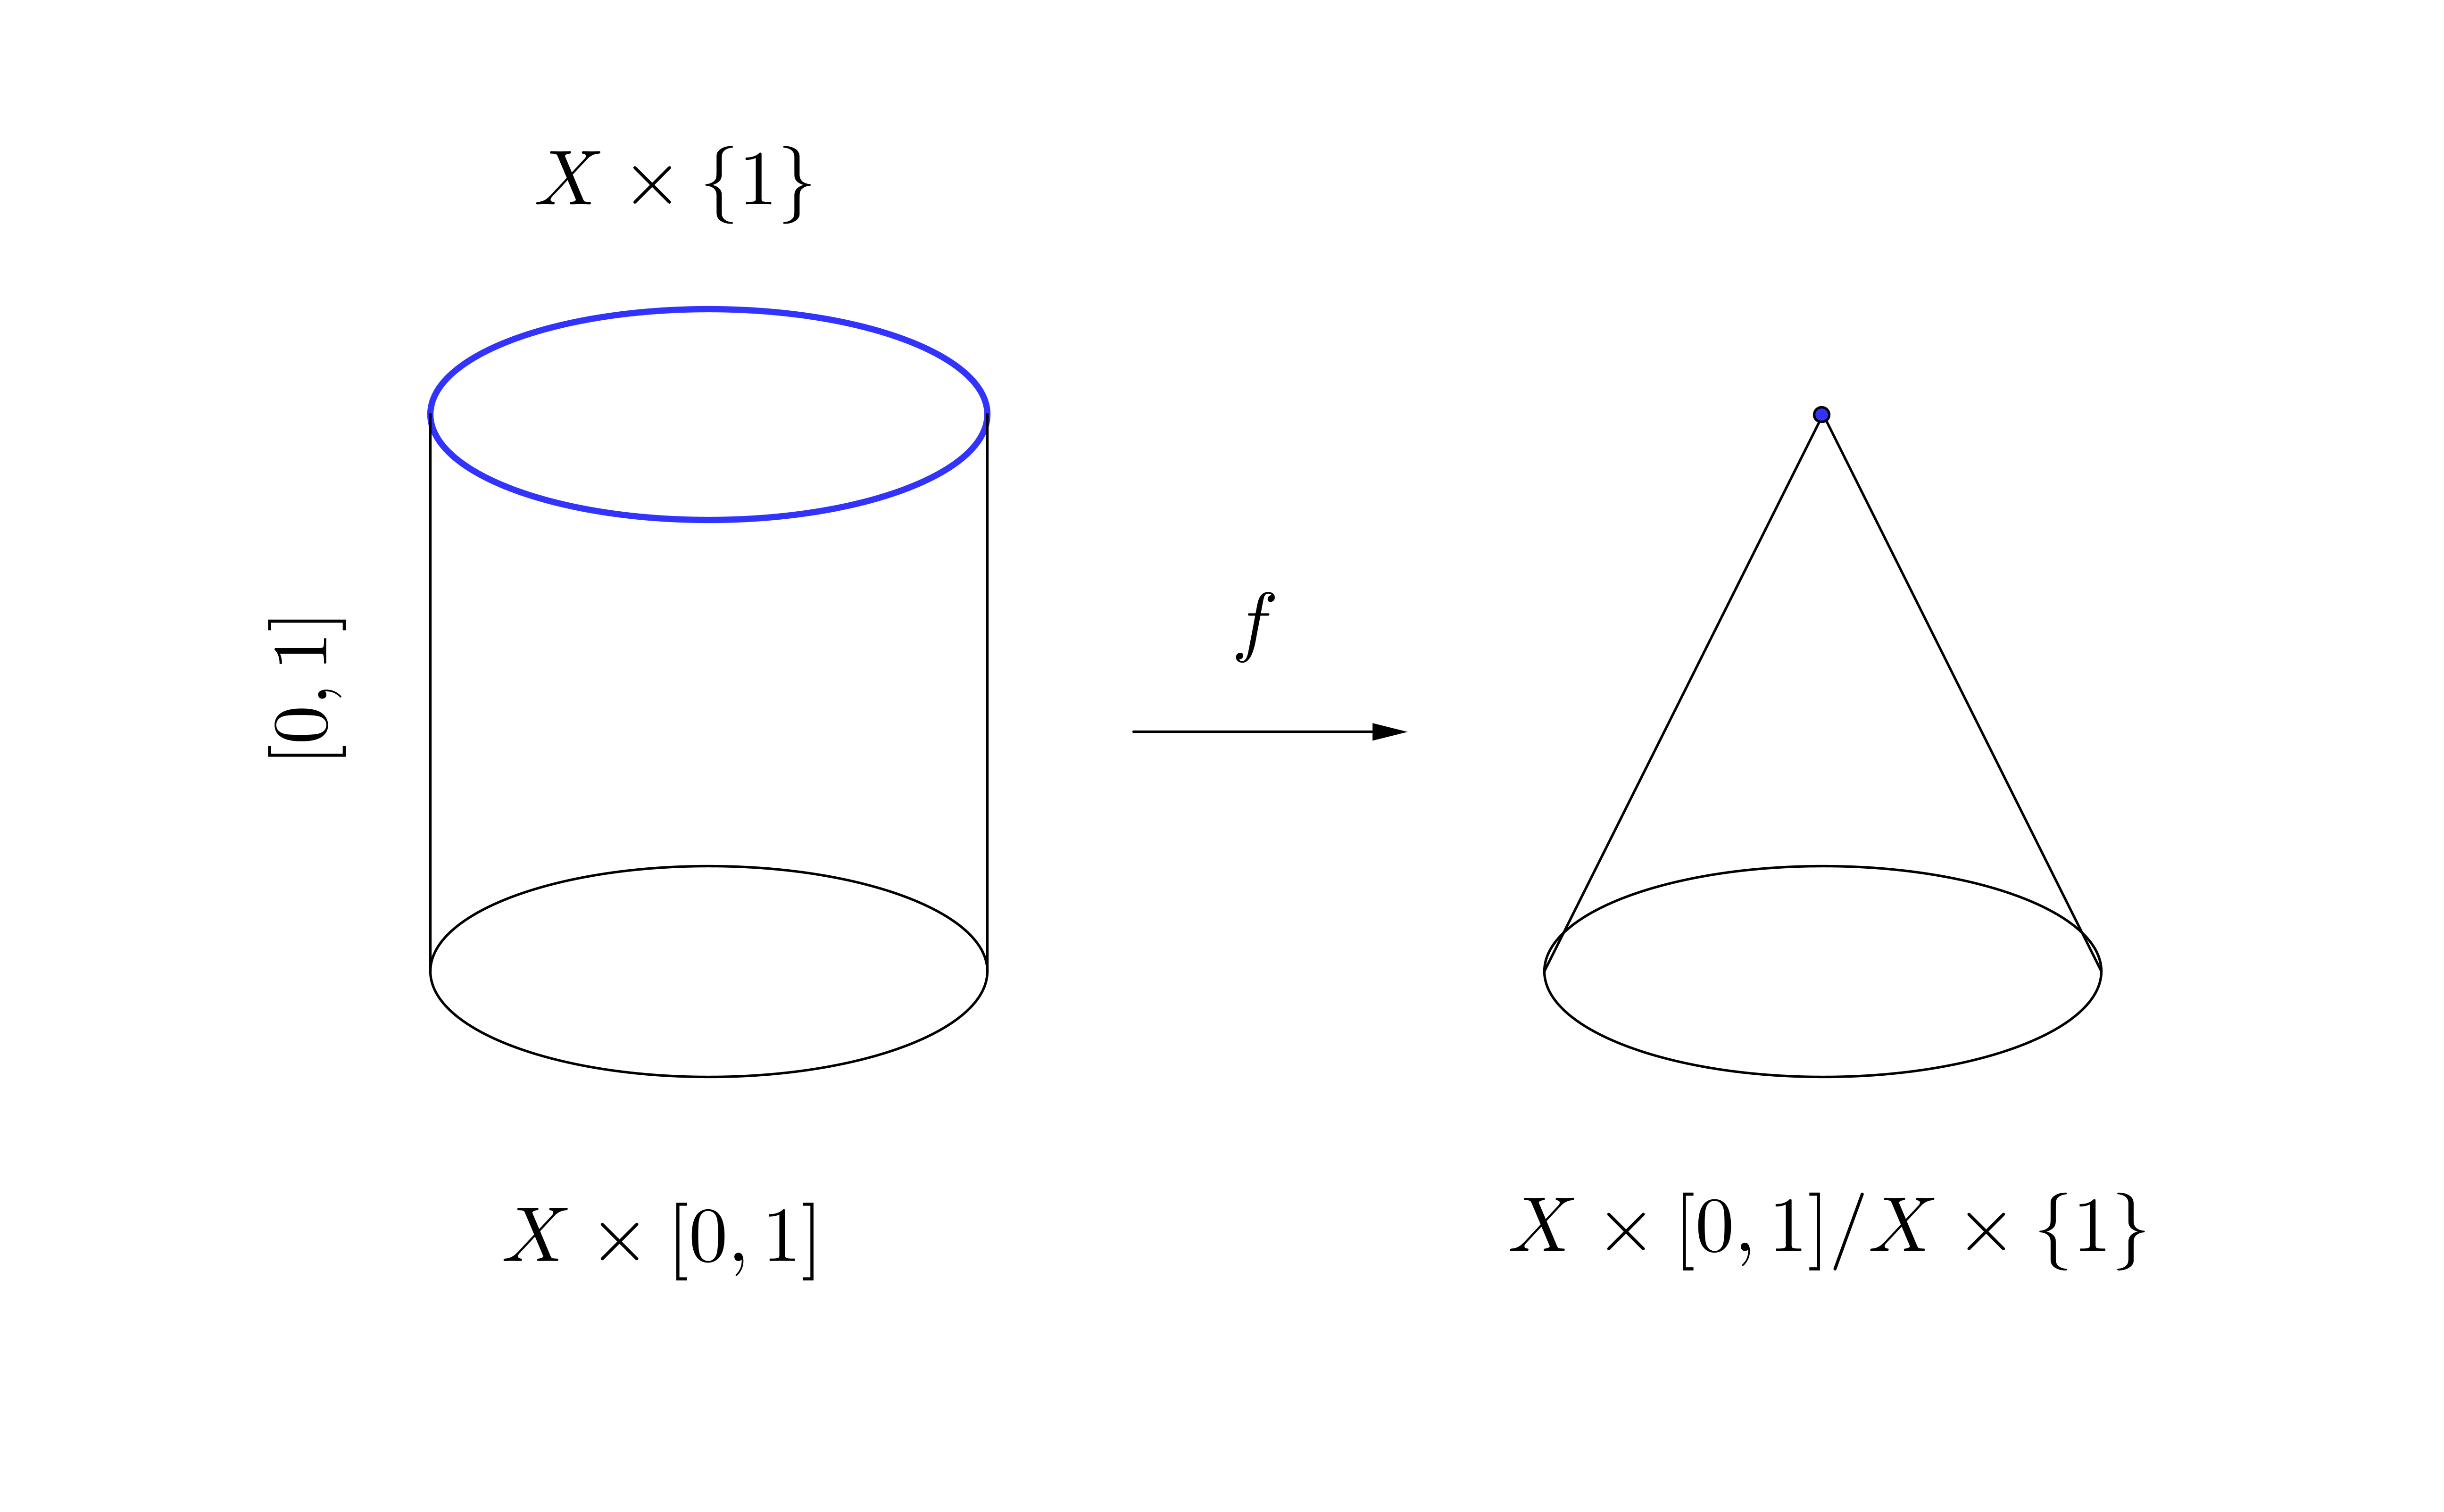
\includegraphics[width=.6\textwidth]{cone.png}
	\caption{A topological cone}%
	\label{figure: topological cone}
\end{wrapfigure}


\begin{definition}[Topological cone]
	The \indexbf{topological cone} of $X$ is defined as $\indexmath[CX]{\mathrm CX} := X \times [0, 1] / X \times \{1\}$.
\end{definition}

Fig.~\ref{figure: topological cone} illustrates a topological cone.

\begin{definition}[Gluing]
	$X$ and $Y$ are both subspaces of $Z$, $f$ is a surjective map from $X$ to $Y$ ($f(X) = Y$). 
	Define $\sim_f$ on $Z$ as: $x \sim y \iff x = y \vee y = f(x)$.
	Then $\indexmath[Z f]{Z_f} := Z/\sim_f$ is called the \indexbf{gluing} of $X$ and $Y$ along $f$.
\end{definition}

\chapter{Topological Manifolds}

\backmatter{}
\nocite{*} % 这个表示列出所有没有在文中被引用的参考文献
\printbibliography[heading=bibliography, title={bibliography}]

\indexprologue{Here listed the important symbols used in this notes}
\printindex[symbol]

\printindex
% \printbibliography
\end{document}